\newcommand{\AND}{\texttt{AND}\xspace}
\newcommand{\RST}{\texttt{RST}\xspace}
\newcommand{\CLK}{\texttt{CLK}\xspace}
\newcommand{\HOLDN}{\texttt{HOLDN}\xspace}
\newcommand{\MULI}{\texttt{MULI}\xspace}
\newcommand{\MULO}{\texttt{MULO}\xspace}
\newcommand{\infer}{\texttt{infer}\xspace}
\newcommand{\multype}{\texttt{multype}\xspace}
\newcommand{\pipe}{\texttt{pipe}\xspace}
\newcommand{\mac}{\texttt{mac}\xspace}
\newcommand{\STDV}{\texttt{STD\_LOGIC\_VECTOR}\xspace}

\subsection{Multiplier}


\subsubsection{Wallace Tree Multiplier}
\label{sec:wallace}

For this project it was decided the most appropriate multiplier scheme would be the Wallace Tree Multiplier. The most important reason for this choice is due to its great performance although at the cost of gates and area.

The Wallace tree is a regular hardware structure to multiply two operands.
It was invented by Chris Wallace, an Australian Computer Scientist in 1964.

The algorithm can be divided in three major steps:
\begin{enumerate}
\item The initial \AND operation between all combinations of bits of each operand. The weights must be adjusted according to the location of the operands, just like in the classical pen-and-paper algorithm. The resulting tree, using dot notation, is shown in figure~\ref{fig:wallace_tree}.

\begin{figure}[H]
\centering
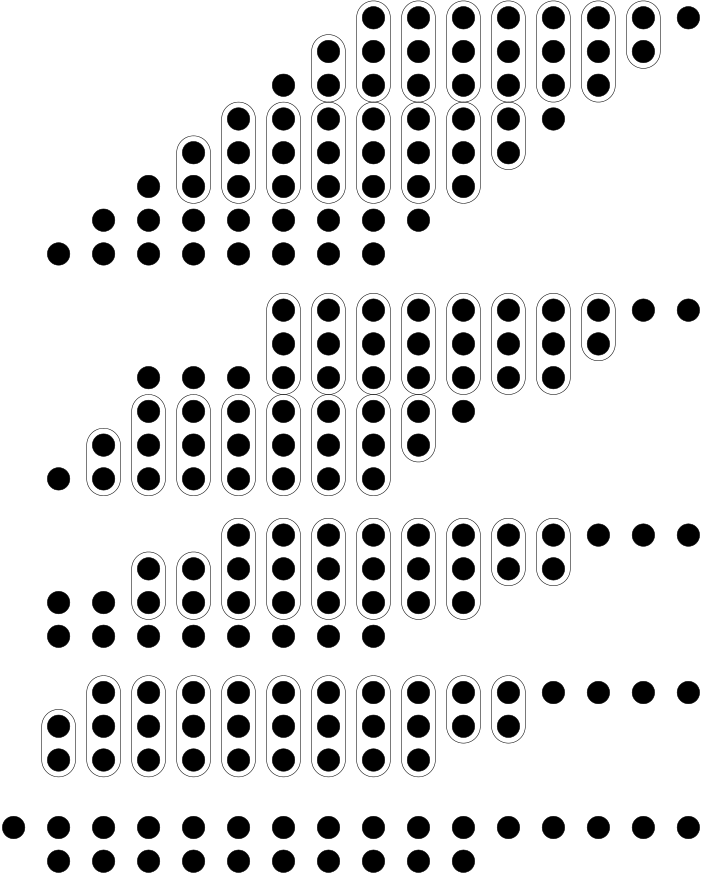
\includegraphics[width=0.70\textwidth,height=0.4\textheight,keepaspectratio]{Wallace_tree.png}
\caption{Resulting tree after executing step 1 for and 8 bit by 8 bit multiplication.}
\label{fig:wallace_tree}
\end{figure}

\item Thereafter the tree must be reduced through the use of half adders and full adders. These will convert each two or three ``dots'', respectively, into one and a carry out for the following column. This step shall be iterated sufficient times until only two numbers emerge.

\item Finally, the two remaining numbers can be summed with a conventional adder. The width of the result should be equal to the sum of the widths of the original operators. For example for a 32 bit times 32 bit operation, the result shall be 64 bits wide. 
\end{enumerate}  

For our particular implementation the aforementioned description was modified to accommodate signed numbers through the use of the modified Baugh-Wooley algorithm. The details of this alteration will be explained in section~\ref{sec:implementation}.

\subsubsection{Advantages and Disadvantages}

The main advantages of this scheme are the speed obtained and regular mapping in hardware. The structure of the tree is consistent throughout the several steps. On the other hand, this design is costly in the amount of gates necessary and total area. The latter can be improved by reorganizing the tree for efficiency. The `waste' in the traditional structure is particularly noticeable on the extremes of each line of the tree, as shown in figure~\ref{fig:paper_wastedarea}. \cite{betterwallace} details possible techniques that can be implemented to tackle this issue and reduce the area cost of the Wallace multiplier. The main idea is to split the tree into two overlapping trees, hence saving area. Thereafter the additions take place in opposite directions. 
However due to lack of time it was not possible to implement the proposed ideas on the multiplier.

\begin{figure}[H]
\centering

\subfloat[Detail of Wallace Tree from~\cite{betterwallace}. It is clearly visible a significant percentage of unused area.]{\label{fig:paper_wastedarea}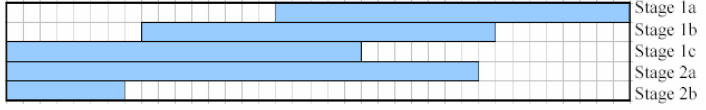
\includegraphics[width=0.85\textwidth,height=0.2\textheight,keepaspectratio]{paper_wastedarea.png}}\\
\subfloat[Modified Wallace Tree from~\cite{betterwallace}. The image reflects the better area utilization based on the algorithm present in the paper.]{\label{fig:paper_improvedarea}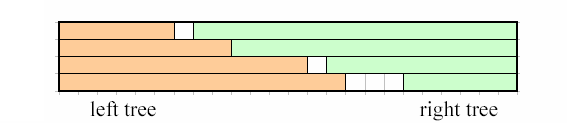
\includegraphics[width=0.85\textwidth,height=0.2\textheight,keepaspectratio]{paper_improvedarea.png}}
\caption{Wallace tree structure before and after the reorganization.}
\label{fig:paper}
\end{figure}


\subsubsection{Implementation and Simulation Results}
\label{sec:implementation}

This section will be used to introduce the reader to the implementation requirements for the multiplier. Followed by a simple, high-level description of the architecture used to accomplish them.

The implementation tries to closely mimic the three algorithm steps. However additional signals are necessary for the correct interface with the processor. According to the documentation~\cite{doc}~and~\cite{doc2}, there are 3 input signals, \RST, \CLK and \MULI and 1 output signal \MULO. Moreover, there are 4 generics: \infer, \multype, \pipe and \mac. \MULI includes the 32 bit operands (along with an extra signal bit), and severals flag to request flushing of the current operation, indicate signed multiplication, to initiate, and to start multiply and accumulate. On the other hand \MULO includes a self explanatory ready signal, a nready signal (not used), condition codes that reflect if the result is zero or negative and finally the 64 bit result.

The most significant generic is multype that configures the multiplier to different operand's sizes. These are 16x16, 32x8, 32x16 and 32x32. It is important to note that a discrepancy between the documentation and the actual code exists regarding the multiplier. The infer generic has been replace by tech (related to the target architecture) in the original VHDL file: \texttt{mul32.vhd}. Our custom multiplier replicates this configuration.

As mentioned in~\ref{sec:wallace} the algorithm can be divided in three major parts.

On part 1 the operands are \texttt{AND}ed together and their weights are adjusted. To reflect this a three dimensional \STDV was created and named \texttt{WallaceTree}. The first dimension reflects the number of stages (or levels) necessary to finish the operation. These values are computed offline for the four multype possibilities. The second dimension relates to the number of `lines' of the matrix, or its height. The range is always equal to the width of the first operand. Finally, the third dimension accounts for the number of columns, or its width, which is necessarily equal to the sum of the width's of each operand. In practice the 3D array was converted to 1D as synthesis tools have better support for the latter, nonetheless the same principles stand.

To be able to multiply signed operands the modified Baugh-Wooley multiplication was used (\emph{cf.}~\cite{part3}). Therefore some values are complemented if the input is signed. Moreover on the final step a constant value is added to the two operands.
This action completes the first step.

Thereafter each group of 3 or 2 bits must be compressed to 1, using full-adders and half-adders respectively. If an odd number of bits exist in a certain column the last bit is transfered to the next level. Repeating this process sufficient times\footnote{The exact number of iterations required can be inferred from the integer constant \texttt{levels} previously mentioned.}, the height of the matrix is reduced to 2. These can be added with a conventional adder to determine the final result.

To help with these operations the exact number of full-adders and half-adders for each column of each stage were precomputed. Moreover two other constants arrays exist that indicate the number of carry ins each column receives and if it has a remainder bit (odd numbered of lines).
Having this information the location of the appropriate inputs (x, y and carry in for the full adder) and outputs (s and carry out) are mapped to a full (or half) adder instance to determine the result.

Step 3 is simply an addition with the first two `lines' of the last stage of the \texttt{WallaceTree} signal. However, if the multiplication is signed an extra \STDV is added to these, as explained in~\cite{part3}.

The extra signals indicate the result is ready and the condition codes are updated to reflect the result of the operation.  
The evolution of the signals driven by our testbench is shown in~\ref{fig:mul32_wave}.


\begin{figure}[H]
\centering
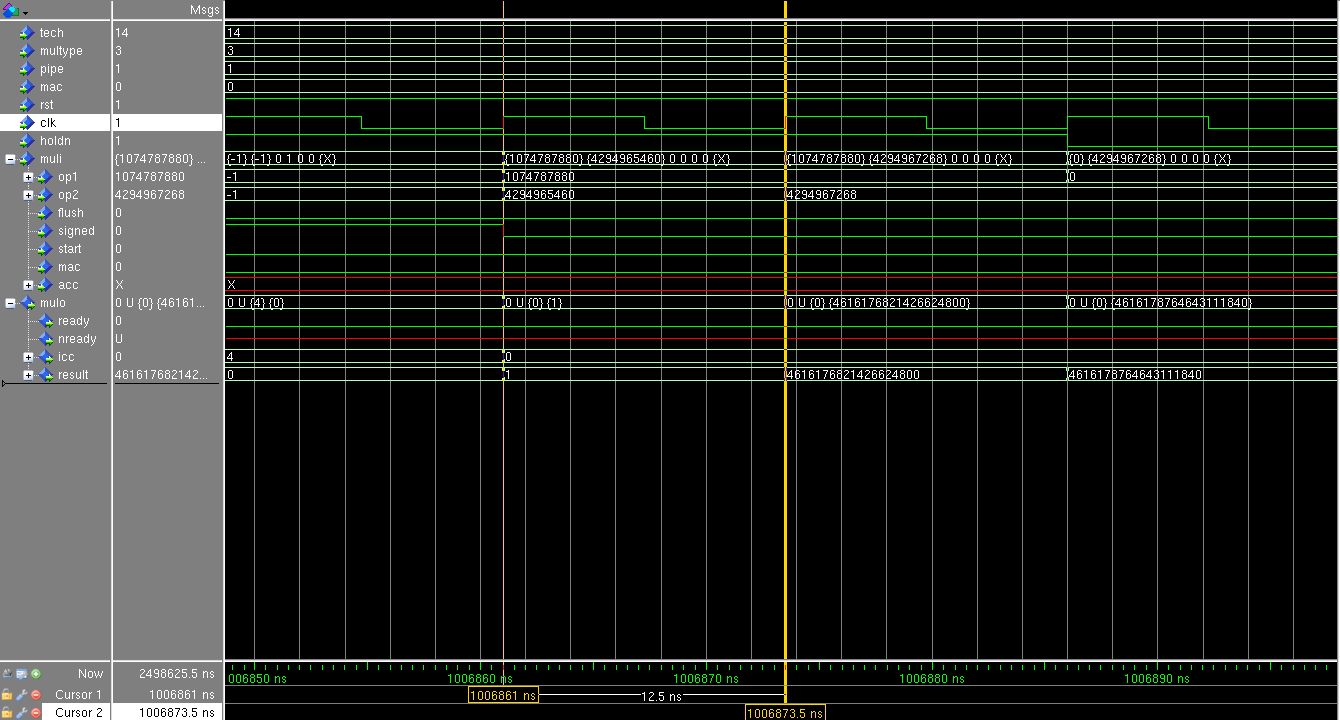
\includegraphics[width=1\textwidth,height=0.4\textheight,keepaspectratio]{mul32_wave.png}
\caption{Screenshot of the Modelsim's Wave for the multiplier. For this particular simulation a 32x32 operation is shown, along with all the appropriate signals.}
\label{fig:mul32_wave}
\end{figure}